          \vspace{1em}
    \centering
    \begin{minipage}{0.7\linewidth}
    \begin{columns}
        \begin{column}{0.5\textwidth}
        \centering
        \colorbox{cyan}{
      \begin{minipage}{6.0cm}
        \centering
        $\underset{\text{continuous losses}}{v < v_\text{cut}}$
    \end{minipage}
      }
        \end{column}

        \begin{column}{0.5\textwidth}
        \centering
        \colorbox{orange}{
      \begin{minipage}{6.0cm}
          \centering
        $\underset{\text{stochastic losses}}{v > v_\text{cut}}$
    \end{minipage}
      }
        \end{column}
    \end{columns}
    \end{minipage}

    \vspace{-3em}


  \centering
    \begin{tcolorbox}[colback=light-gray,colframe=black,width=0.8\linewidth]
    \begin{figure}
      \normalsize
      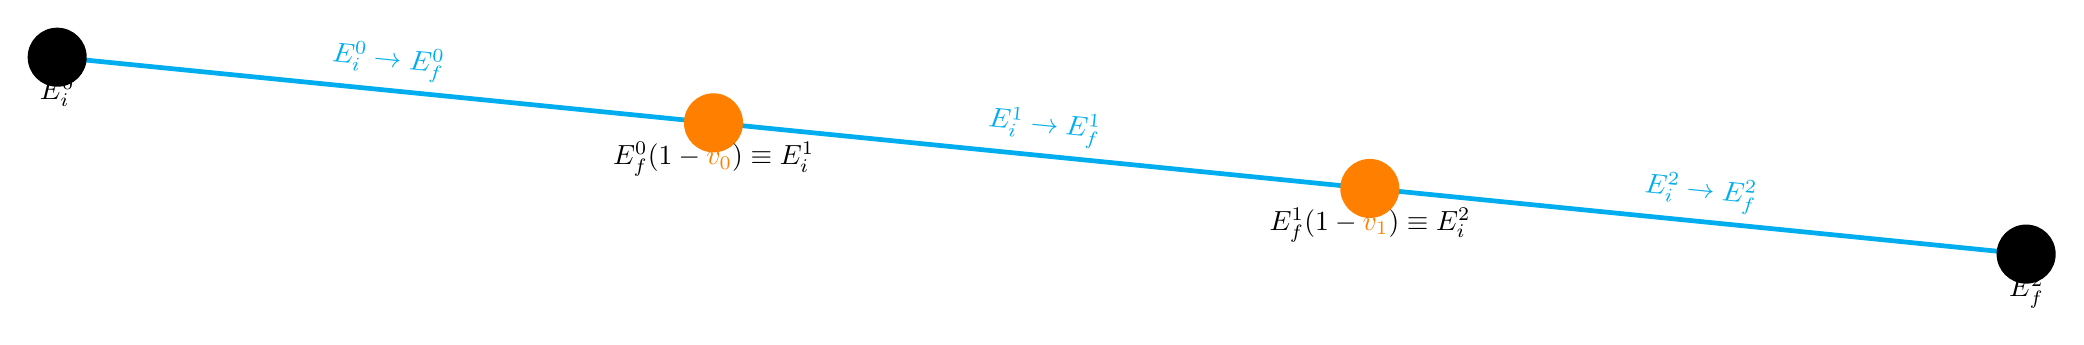
\begin{tikzpicture}[scale=2.50]
        \centering
            \coordinate (E0) at (0,0);
            \coordinate (E1) at (1/3 * 10, -1/3 * 1);
            \coordinate (E2) at (2/3 * 10, -2/3 * 1);
            \coordinate (E3) at (10, -1);

      \draw [cyan, line width=0.6mm] (E0) -- (E1) node[pos=0.5, sloped, above] {$E_i^0 \rightarrow E_f^0$};
      \draw [cyan, line width=0.6mm] (E1) -- (E2) node[pos=0.5, sloped, above] {$E_i^1 \rightarrow E_f^1$};
      \draw [cyan, line width=0.6mm] (E2) -- (E3) node[pos=0.5, sloped, above] {$E_i^2 \rightarrow E_f^2$};

      \fill [black] (E0) circle (0.15) node[label=below: $E_{i}^0$]{};
      \fill [orange] (E1) circle (0.15) node[label=below: $\color{black} E_{f}^0 (1 - \textcolor{orange}{v_0}) \equiv E_i^1$]{};
      \fill [orange] (E2) circle (0.15) node[label=below: $\color{black} E_{f}^1 (1 - \textcolor{orange}{v_1}) \equiv E_i^2$]{};
      \fill [black] (E3) circle (0.15) node[label=below: $\color{black} E_{f}^2$]{};


      \end{tikzpicture}
    \end{figure}
    \end{tcolorbox}
    \vspace{-3em}
    \begin{minipage}{0.9\linewidth}
    \Large
    \begin{columns}[onlytextwidth]
      \begin{column}{0.5\textwidth}  
        \centering
        $\displaystyle\int_{E_i}^{E_f} \frac{\sigma\left(E\right)}{-f\left(E\right)} \cdot \mathrm{d}E = -\log{\left( \xi \right)}$
      \end{column}
      \begin{column}{0.5\textwidth}
        \centering
        $v_\text{cut} = \text{min}\left[\sfrac{e_\text{cut}}{E}, v\prime_\text{cut}\right]$  
      \end{column}
    \end{columns}
    \end{minipage}